\documentclass[11pt,a4paper]{report}

% ---------------------------------------------------------------------------
% Packages
% ---------------------------------------------------------------------------
\usepackage[margin=2.6cm]{geometry}
\usepackage[utf8]{inputenc}
\usepackage[T1]{fontenc}
\usepackage{amsmath}
\usepackage{graphicx}
\usepackage{booktabs}
\usepackage{xcolor}
\usepackage{tcolorbox}
\usepackage{tikz}
\usepackage{pgfplots}
\pgfplotsset{compat=1.18}
\usepackage{fontawesome5}
\usetikzlibrary{arrows.meta, positioning, shapes.geometric, fit, backgrounds}
\usepackage[colorlinks=true, linkcolor=black, citecolor=black, urlcolor=blue!50!black]{hyperref}
\usepackage{caption}
\usepackage{enumitem}
\usepackage{parskip}
\usepackage{pifont}

% ---------------------------------------------------------------------------
% Okabe-Ito colorblind-safe palette
% ---------------------------------------------------------------------------
\definecolor{oiBlack}{HTML}{000000}
\definecolor{oiOrange}{HTML}{E69F00}
\definecolor{oiSkyBlue}{HTML}{56B4E9}
\definecolor{oiGreen}{HTML}{009E73}
\definecolor{oiYellow}{HTML}{F0E442}
\definecolor{oiBlue}{HTML}{0072B2}
\definecolor{oiVermillion}{HTML}{D55E00}
\definecolor{oiPurple}{HTML}{CC79A7}

\definecolor{diffadd}{HTML}{1B7F3B}
\definecolor{diffdel}{HTML}{C0392B}
\definecolor{codebg}{HTML}{F5FAFF}
\definecolor{codeframe}{HTML}{2E75B6}

% ---------------------------------------------------------------------------
% Shared TikZ styles (used across figures for a consistent look)
% ---------------------------------------------------------------------------
\tikzset{
  stagebox/.style={
    draw, rounded corners, thick,
    minimum width=2.3cm, minimum height=1.7cm,
    align=center, font=\small
  },
  phase/.style={
    circle, draw=black, thick, fill=#1,
    text=white, font=\bfseries\small,
    minimum size=8mm, align=center
  },
  procstep/.style={
    draw=#1, thick, rounded corners, fill=#1!8,
    minimum width=3.0cm, minimum height=1.15cm,
    align=center, font=\small, inner sep=4pt
  },
  grouplabel/.style={font=\bfseries\normalsize, text=#1!70!black},
  arr/.style={-{Latex[length=2.5mm]}, thick},
  arrc/.style={-{Latex[length=2.5mm]}, thick, #1},
  bigarr/.style={-{Latex[length=3mm]}, ultra thick, dashed, #1}
}

\captionsetup{font=small, labelfont=bf}

\title{\textbf{Reading Egyptian Hieroglyphs Automatically:\\
A Technical Report on the Design, Machine Learning Methods, and\\
Engineering Issues of a Photo-to-Gloss Pipeline}}
\author{Delfin Eryilmaz}
\date{\today}

\begin{document}

\maketitle

\begin{abstract}
\noindent
This report explains, from first principles, how a piece of software takes a
photograph of Egyptian hieroglyphs and produces, for every sign in the photo,
its Gardiner sign-list code, its transliteration (when one is known), and an
English gloss. The report assumes no prior knowledge of machine learning: every
technical term (neural network, convolution, transfer learning, object
detection, fine-tuning) is defined the first time it is used, and each
definition is followed by a concrete example drawn from this project. The
system is built from three stages that run one after another: finding where
each glyph sits in the photograph (segmentation), deciding which of 171 known
signs each glyph is (classification), and assembling the results into a
readable output (reading-order sorting and dictionary lookup). Two
implementations of the first stage are covered in detail: a classical
image-processing approach that needs no training data, and a newer approach
that fine-tunes a pretrained neural network on synthetically generated
training images. The report also documents a real defect that was found and
fixed during the development of the second approach, as a worked example of
how a plausible-looking machine learning pipeline can fail for a subtle
reason that only becomes visible when it is actually run.
\end{abstract}

\tableofcontents

% =============================================================================
\chapter{Introduction}
% =============================================================================

\section{What this project does}

The input to this system is an ordinary photograph containing one or more
Egyptian hieroglyphic signs, for example a photograph of a carved wall, a
papyrus, or a single inscribed object. The output is a list, one entry per
sign found in the photograph, each entry giving:

\begin{enumerate}[label=(\arabic*)]
  \item the sign's \textbf{Gardiner code}, a short alphanumeric label such as
    \texttt{D21} or \texttt{G17} that Egyptologists use to refer to a specific
    hieroglyphic sign, following the classification scheme published by Sir
    Alan Gardiner in 1927 and still in standard use today;
  \item the sign's \textbf{transliteration}, a short sequence of Latin letters
    approximating how the sign was pronounced or the sound value it
    represents, when one is recorded for that sign (many signs, called
    determinatives, carry meaning but no sound and genuinely have no
    transliteration);
  \item the sign's \textbf{English gloss}, a short English word or phrase
    describing what the sign means.
\end{enumerate}

It is important to state plainly what the system does \emph{not} do. It does
not produce a fluent English sentence translation of an inscription.
Translating hieroglyphic text into readable English requires knowledge of
Middle Egyptian grammar (word order, verb conjugation, determinative
conventions) that a per-sign lookup table cannot supply, and no large corpus
of hieroglyphic text paired with human-translated English sentences exists to
train such a system on. The output is honestly presented as what it is: a
list of individual sign meanings in the order the signs were read, not a
sentence.

\section{Why this is a machine learning problem}

A photograph of a hieroglyph is, to a computer, nothing more than a grid of
numbers: each pixel is stored as one or more numbers describing its
brightness and color. Section~\ref{sec:images-as-numbers} explains this
representation in detail. The task of turning that grid of numbers into
``this is sign D21, the mouth glyph'' cannot be solved by writing an explicit
rule such as ``if the pixels form this exact shape, it is D21'', because
photographs of the same sign vary enormously: different carvings, different
lighting, different camera angles, and different amounts of weathering all
change the exact pixel values while the sign's identity stays the same.
Machine learning is the family of techniques used when the mapping from
input to output is too complex and too variable to write down as an explicit
rule by hand, and is instead learned automatically from many labeled
examples. Section~\ref{sec:what-is-ml} defines this more precisely.

\section{Report roadmap}

Figure~\ref{fig:research-flow} shows the shape of this report at a glance.
Chapter~\ref{ch:background} builds up the machine learning vocabulary used
throughout the rest of the report, starting from what an image looks like to
a computer and ending at convolutional neural networks, the specific kind of
neural network this project uses. Chapter~\ref{ch:segmentation} covers the
first pipeline stage, finding where the glyphs are in a photograph, including
both the classical (non-learned) approach already in production and a newer
approach, still being trained at the time of writing, that fine-tunes a
neural object detector. Chapter~\ref{ch:classification} covers the second
stage, identifying which of the 171 known signs each found glyph is.
Chapter~\ref{ch:assembly} covers how the pipeline puts the per-glyph results
back together into an ordered, human-readable list. Chapter~\ref{ch:demo}
describes the web application built on top of the pipeline.
Chapter~\ref{ch:limitations} states, without softening, what the system does
not yet do well and why.

\begin{figure}[t]
\centering
\begin{tikzpicture}[
  stage/.style={
    draw, rounded corners, thick,
    minimum width=2.3cm, minimum height=1.8cm,
    align=center, font=\small
  }
]

\node[stage] (photo) {\Large\faCamera\\[4pt] Photograph};
\node[stage, right=0.9cm of photo]    (seg)   {\Large\faVectorSquare\\[4pt] Find Each\\Glyph};
\node[stage, right=0.9cm of seg]   (cls) {\Large\faBrain\\[4pt] Identify\\Each Sign};
\node[stage, right=0.9cm of cls] (order)   {\Large\faSortAmountDown\\[4pt] Order the\\Signs};
\node[stage, right=0.9cm of order]    (out)    {\Large\faBook\\[4pt] Look Up \&\\Report};

\draw[arr] (photo) -- (seg);
\draw[arr] (seg) -- (cls);
\draw[arr] (cls) -- (order);
\draw[arr] (order) -- (out);

\end{tikzpicture}
\caption{The five stages this report walks through, from an input photograph
to the final list of Gardiner codes, transliterations, and glosses. Each
stage is a separate chapter or section below.}
\label{fig:research-flow}
\end{figure}

% =============================================================================
\chapter{Background: How a Computer ``Sees'' and ``Learns''}
\label{ch:background}
% =============================================================================

This chapter defines every piece of machine learning vocabulary used
elsewhere in the report. A reader already familiar with neural networks and
convolutional neural networks can skip to Chapter~\ref{ch:segmentation}
without losing anything needed later.

\section{Images as numbers}
\label{sec:images-as-numbers}

A digital photograph is stored as a grid of small squares called pixels.
Each pixel holds one number (for a grayscale image, where the pixel is some
shade between black and white) or three numbers (for a color image, one each
for red, green, and blue light intensity). A typical grayscale pixel value
runs from 0 (pure black) to 255 (pure white); a mid-gray pixel might be 128.
A small grayscale image, say 50 pixels wide by 75 pixels tall, is therefore
nothing more than a table of $50 \times 75 = 3{,}750$ numbers between 0 and
255. This project's single-glyph training images are exactly that size and
format: 50 by 75 pixel grayscale crops, each pixel a single brightness
number.

This matters because every operation described in this report, whether it is
a classical image-processing step or a neural network, is ultimately doing
arithmetic on these grids of numbers. There is no step at which the computer
``looks at'' the image the way a person does; every stage described below
reduces to additions, multiplications, comparisons, and lookups performed on
a table of numbers.

\section{What machine learning means here}
\label{sec:what-is-ml}

Machine learning, in the specific sense used throughout this report, means
building a function that maps an input (here, a grid of pixel numbers) to an
output (here, a sign identity, or a set of bounding boxes), where the exact
arithmetic that function performs is not written by a programmer but is
instead adjusted automatically based on many examples of correct
input-output pairs. This process of automatic adjustment is called
\textbf{training}. A concrete example used throughout this report: the sign
classifier described in Chapter~\ref{ch:classification} is trained on 4{,}031
single-glyph images, each one labeled with which of 171 Gardiner codes it
is; training adjusts the classifier's internal arithmetic so that, given a
new image it has never seen, it outputs the correct code as often as
possible.

Three terms recur throughout this report and are worth fixing precisely
before they appear again.

\begin{itemize}
  \item \textbf{Training data} is the collection of labeled examples used
    to adjust the model. For the classifier, this is the 4{,}031 labeled
    glyph crops (Section~\ref{sec:the-dataset}). For the object detector
    described in Chapter~\ref{ch:segmentation}, no labeled real-world
    photographs exist, so the training data is synthetically generated
    (Section~\ref{sec:composite-synthesis}).
  \item \textbf{A model} is the function being trained, together with the
    specific numeric values (called \textbf{weights}) it currently holds.
    Two models with the same structure but different weights, for example
    before and after training, behave completely differently.
  \item \textbf{Inference} is the act of running an already-trained model on
    a new input to get an output, as opposed to training, which is the act
    of adjusting the model's weights. Once a model is trained, running it
    on the Streamlit demo application (Chapter~\ref{ch:demo}) is inference,
    not training; no further learning happens at that point.
\end{itemize}

\section{Neural networks, from scratch}
\label{sec:neural-networks}

A \textbf{neural network} is one specific kind of trainable function, loosely
inspired by connections between neurons in a brain, though the analogy
should not be taken literally: the arithmetic involved is ordinary linear
algebra, not a simulation of biological neurons.

A neural network is organized into \textbf{layers}. Each layer is a set of
units, historically called neurons, arranged side by side. The first layer,
the \textbf{input layer}, holds the raw input numbers (for an image, the
pixel values, laid out in some order). The last layer, the \textbf{output
layer}, holds the network's answer (for a classifier choosing among 171
signs, the output layer has 171 units, one per possible sign). Any layers
between the input and output are called \textbf{hidden layers}.

Every unit in one layer is connected to every unit in the next layer by a
\textbf{weight}, a single adjustable number. A unit's value is computed as a
weighted sum of every unit's value in the previous layer (each multiplied by
its connecting weight and added together), passed through a simple nonlinear
function called an \textbf{activation function} that decides how strongly
the unit ``fires''. Figure~\ref{fig:neural-network} shows this structure for
a small example network. \textbf{Training} a neural network means searching
for the specific set of weight values that makes the network's output layer
agree with the correct label as often as possible across the training data,
using an algorithm called backpropagation combined with gradient descent;
this project does not implement that search algorithm itself, since it is
provided by the PyTorch library, but the report returns to what is actually
being adjusted (Section~\ref{sec:transfer-learning}) when it discusses how
the sign classifier is trained.

\begin{figure}[t]
\centering
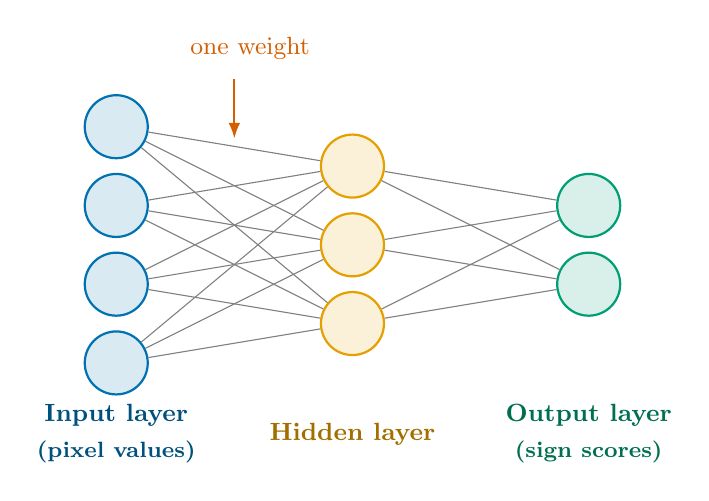
\begin{tikzpicture}[
  neuron/.style={circle, draw, thick, minimum size=8mm},
  inlayer/.style={neuron, fill=oiBlue!15, draw=oiBlue},
  hidlayer/.style={neuron, fill=oiOrange!15, draw=oiOrange},
  outlayer/.style={neuron, fill=oiGreen!15, draw=oiGreen},
  layerlabel/.style={font=\small\bfseries, align=center}
]

% Input layer
\node[inlayer] (i1) at (0,3) {};
\node[inlayer] (i2) at (0,2) {};
\node[inlayer] (i3) at (0,1) {};
\node[inlayer] (i4) at (0,0) {};
\node[layerlabel, text=oiBlue!70!black] at (0,-0.9) {Input layer\\[2pt]\footnotesize(pixel values)};

% Hidden layer
\node[hidlayer] (h1) at (3,2.5) {};
\node[hidlayer] (h2) at (3,1.5) {};
\node[hidlayer] (h3) at (3,0.5) {};
\node[layerlabel, text=oiOrange!70!black] at (3,-0.9) {Hidden layer};

% Output layer
\node[outlayer] (o1) at (6,2) {};
\node[outlayer] (o2) at (6,1) {};
\node[layerlabel, text=oiGreen!70!black] at (6,-0.9) {Output layer\\[2pt]\footnotesize(sign scores)};

% Connections input -> hidden
\foreach \i in {i1,i2,i3,i4}
  \foreach \h in {h1,h2,h3}
    \draw[gray, thin] (\i) -- (\h);

% Connections hidden -> output
\foreach \h in {h1,h2,h3}
  \foreach \o in {o1,o2}
    \draw[gray, thin] (\h) -- (\o);

% Weight callout
\draw[oiVermillion, thick, -{Latex[length=2mm]}] (1.5,3.6) -- (1.5,2.85);
\node[oiVermillion, font=\small, align=center] at (1.7,4.0) {one weight};

\end{tikzpicture}
\caption{A small neural network with one input layer (4 units), one hidden
layer (3 units), and one output layer (2 units). Every line is a weight, a
number adjusted during training. A real classifier layer in this project has
far more units per layer than shown here; the structure is the same, only
the size differs.}
\label{fig:neural-network}
\end{figure}

\subsection*{Worked example}

Suppose, for illustration, a tiny network is being trained to tell apart two
signs using only 4 input numbers (a drastically simplified stand-in for
pixel values) and the 2-unit output layer shown in
Figure~\ref{fig:neural-network}. Before training, the weights are set to
small random numbers, so the network's two output units produce essentially
random scores for any input. Training repeatedly shows the network a labeled
example (an input together with which of the two signs it actually is),
compares the network's output to the correct answer, and nudges every weight
in the network slightly in the direction that would have made the output
closer to correct for that example. Repeated over thousands of examples,
this nudging process converges on a set of weights where the correct output
unit tends to score highest for the corresponding input. The single arrow
labeled ``one weight'' in Figure~\ref{fig:neural-network} is one such
adjustable number; a real network in this project has hundreds of thousands
of them, but the training principle (compare to a labeled example, nudge
every weight slightly) is unchanged.

\section{Convolutional neural networks}
\label{sec:cnn}

The network described in Section~\ref{sec:neural-networks} connects every
input unit to every hidden unit. Applied directly to an image, this becomes
impractical almost immediately: a modest 224 by 224 pixel color image has
$224 \times 224 \times 3 = 150{,}528$ input numbers, and a hidden layer of a
useful size would need tens of millions of weights just for the first layer,
most of which would be redundant, since a pattern that identifies a curved
stroke in the top-left corner of an image is, for the most part, the exact
same pattern that would identify a curved stroke anywhere else in the image.

A \textbf{convolutional neural network}, or \textbf{CNN}, solves this by
reusing the same small set of weights at every position in the image,
instead of learning a separate weight for every pixel-to-unit connection. A
small grid of weights, called a \textbf{filter} or \textbf{kernel} (typically
as small as $3\times3$ pixels), is slid across the entire input image. At
every position, the filter's weights are multiplied against the pixels
currently underneath it and summed into a single number; sliding the filter
across the whole image produces a grid of these summed numbers called a
\textbf{feature map}. Because the same filter is reused everywhere, a filter
that has learned to respond strongly to (for example) a horizontal edge will
detect horizontal edges anywhere in the image, using a tiny fraction of the
weights a fully-connected layer would need. A convolutional layer normally
learns many filters at once (tens to hundreds), each producing its own
feature map, so that different filters can specialize in detecting different
simple patterns (edges at different angles, corners, small textures).

CNNs stack many convolutional layers on top of each other. Layers close to
the input tend to learn simple, general-purpose patterns such as edges and
corners; feature maps from an early layer feed into a later convolutional
layer, whose filters combine those simple patterns into more complex ones
(for example, a curve plus a straight edge might combine into something
resembling part of a bird's beak); layers near the end of the network
combine complex patterns into whole-object concepts. Between convolutional
layers, a \textbf{pooling} step commonly shrinks each feature map (for
example, by keeping only the largest value in each small block of the map),
which reduces the amount of computation needed by later layers and makes the
network somewhat tolerant to small shifts in where a pattern appears.
Figure~\ref{fig:cnn} shows this structure end to end, from an input image to
a final classification.

\begin{figure}[t]
\centering
\begin{tikzpicture}[
  grouplabel/.style={font=\bfseries\normalsize, text=#1!70!black},
  procstep/.style={
    draw=#1, thick, rounded corners, fill=#1!8,
    minimum width=2.6cm, minimum height=1.15cm,
    align=center, font=\small, inner sep=4pt
  }
]

\node[grouplabel=oiBlue] (t1) at (0,2.6) {Feature Extraction};
\node[phase=oiBlue!70!black] (p1) at (0,1.9) {1};

\node[procstep=oiBlue] (img) at (0,0.6) {\Large\faImage\\[2pt] Input\\Image};
\node[procstep=oiBlue, right=6mm of img] (conv1) {\Large\faThLarge\\[2pt] Convolution\\Filters};
\node[procstep=oiBlue, right=6mm of conv1] (pool1) {\Large\faCompress\\[2pt] Pooling};
\node[procstep=oiBlue, right=6mm of pool1] (conv2) {\Large\faThLarge\\[2pt] More\\Filters};

\draw[arrc=oiBlue] (img) -- (conv1);
\draw[arrc=oiBlue] (conv1) -- (pool1);
\draw[arrc=oiBlue] (pool1) -- (conv2);

\node[procstep=oiGreen!45!black, below=16mm of img] (flat) {\Large\faStream\\[2pt] Flatten};
\node[procstep=oiGreen!45!black, right=6mm of flat] (fc) {\Large\faProjectDiagram\\[2pt] Fully\\Connected};
\node[procstep=oiGreen!45!black, right=6mm of fc] (out) {\Large\faTags\\[2pt] Sign\\Scores};

\node[grouplabel=oiGreen!45!black, above=3mm of flat] (t2) {Classification};
\node[phase=oiGreen!35!black, left=3mm of t2] (p2) {2};

\draw[arrc=oiBlue, -{Latex[length=2.5mm]}] (conv2.south) -- ++(0,-0.9) -| (flat.north);
\draw[arrc=oiGreen!45!black] (flat) -- (fc);
\draw[arrc=oiGreen!45!black] (fc) -- (out);

\end{tikzpicture}
\caption{A convolutional neural network, in two phases. Feature extraction
(blue) repeatedly applies small filters and pooling to build up increasingly
complex patterns from the raw pixels. Classification (green) flattens the
final feature maps into a single list of numbers and passes them through a
fully connected layer (the kind described in
Section~\ref{sec:neural-networks}) to produce one score per possible sign.
The sign classifier in this project, described in
Section~\ref{sec:transfer-learning}, is a CNN of this shape called ResNet18.}
\label{fig:cnn}
\end{figure}

\subsection*{Worked example}

Consider a single $3\times3$ edge-detecting filter with weights arranged so
that it produces a large output when the pixels underneath it go from dark
on the left to light on the right, and a small output otherwise. Sliding
this filter across a photograph of the sign \texttt{D21} (a mouth, drawn as
a horizontal curved shape) produces a feature map that lights up strongly
along the sign's left-facing edges and stays low elsewhere. That feature map
is itself just another grid of numbers, so a second convolutional layer can
be applied to it exactly as the first layer was applied to the original
image, this time detecting combinations of edges rather than raw pixel
contrast. Repeating this a handful of times, exactly as shown in
Figure~\ref{fig:cnn}, is how a CNN builds up from ``this pixel is darker
than its neighbor'' to ``this arrangement of edges and curves looks like a
D21''.

% =============================================================================
\chapter{Finding Each Glyph in a Photograph (Segmentation)}
\label{ch:segmentation}
% =============================================================================

\section{The task: from photograph to bounding boxes}

Before any sign can be identified, the system first has to answer a simpler
question: where in the photograph does each individual sign sit? This is
called \textbf{segmentation} in this project (the more general term in the
wider computer vision field is \textbf{object detection}, discussed in
Section~\ref{sec:detection-vs-classification}). The output of this stage is
a list of \textbf{bounding boxes}, one per glyph found in the photograph. A
bounding box is the smallest upright rectangle that contains one glyph,
stored as four numbers: an $x$ and $y$ position for its top-left corner, and
a width and height. Every later stage of the pipeline (classification,
reading-order sorting, lookup) operates on the region of the photograph
inside one bounding box at a time, never on the whole photograph at once.

This project implements two different ways of producing these bounding
boxes, sharing one common interface (an abstract base class named
\texttt{Segmenter} in the source code) so that either one can be plugged
into the rest of the pipeline without changing anything downstream. The
first, described in Section~\ref{sec:classical-cv}, is a classical
image-processing method that needs no training data and is the one
currently used by default. The second, described in
Section~\ref{sec:trained-detector}, is a neural network trained
specifically to find hieroglyphs, and is expected to perform better on
difficult, real-world photographs once training completes.

\section{A classical computer vision approach}
\label{sec:classical-cv}

The classical segmenter finds glyphs using a fixed sequence of image
processing steps, none of which involve a trained model or any adjustable
weights, only local pixel arithmetic and long-established computer vision
techniques. Figure~\ref{fig:classical-cv} shows the five steps in order.

\begin{figure}[t]
\centering
\begin{tikzpicture}[
  procstep/.style={
    draw=oiBlue, thick, rounded corners, fill=oiBlue!8,
    minimum width=2.7cm, minimum height=1.3cm,
    align=center, font=\small, inner sep=4pt
  }
]

\node[procstep] (gray) {\Large\faImage\\[2pt] Convert to\\Grayscale};
\node[procstep, right=7mm of gray] (blur) {\Large\faSlidersH\\[2pt] Blur to\\Reduce Noise};
\node[procstep, right=7mm of blur] (thresh) {\Large\faAdjust\\[2pt] Binarize\\(Threshold)};
\node[procstep, right=7mm of thresh] (close) {\Large\faObjectGroup\\[2pt] Merge Nearby\\Strokes};
\node[procstep, below=9mm of thresh] (contour) {\Large\faDrawPolygon\\[2pt] Trace\\Outlines};
\node[procstep, right=7mm of contour] (box) {\Large\faVectorSquare\\[2pt] Keep Boxes of\\Plausible Size};

\draw[arrc=oiBlue] (gray) -- (blur);
\draw[arrc=oiBlue] (blur) -- (thresh);
\draw[arrc=oiBlue] (thresh) -- (close);
\draw[arrc=oiBlue] (close.south) -- ++(0,-0.35) -| (contour.north);
\draw[arrc=oiBlue] (contour) -- (box);

\end{tikzpicture}
\caption{The classical segmenter's five processing steps, applied to every
input photograph in order. None of these steps involve a trained model;
every step is a fixed image-processing rule.}
\label{fig:classical-cv}
\end{figure}

\begin{enumerate}[label=(\arabic*)]
  \item \textbf{Convert to grayscale.} If the input photograph has separate
    red, green, and blue channels, they are combined into a single
    brightness channel, since the remaining steps only need brightness, not
    color.
  \item \textbf{Blur to reduce noise.} A small Gaussian blur (averaging each
    pixel with its immediate neighbors) is applied first, so that isolated
    single-pixel speckles of noise do not get mistaken for real detail by
    the next step.
  \item \textbf{Binarize (threshold).} Every pixel is converted to either
    pure black or pure white, based on whether it is darker or lighter than
    a cutoff brightness. The implementation defaults to \textbf{adaptive}
    thresholding, meaning the cutoff is computed separately for each local
    neighborhood of the image (a 25-pixel-wide window, in the current
    configuration) rather than using one single cutoff for the whole photo;
    this copes better with a photograph that is more brightly lit on one
    side than the other, since a single global cutoff would misclassify an
    evenly-lit dark carving as ``all background'' the moment part of the
    photo gets brighter than the cutoff. The method assumes glyphs are
    darker than their surrounding surface, which holds for incised or
    shadowed carvings, the expected common case.
  \item \textbf{Merge nearby strokes.} A single hieroglyphic sign is
    frequently drawn as several separate pen or chisel strokes rather than
    one connected shape. A morphological operation called \textbf{closing}
    (a controlled expansion of the white regions, followed by an equal
    controlled shrink) is applied so that strokes belonging to the same
    glyph, which are usually close together, get merged into one connected
    white blob, while strokes belonging to different, more distant glyphs
    stay separate.
  \item \textbf{Trace outlines and keep plausible boxes.} Every connected
    white blob's outline (its \textbf{contour}) is traced, and the smallest
    upright rectangle containing that outline becomes a candidate bounding
    box. Candidates that are extremely small (likely leftover noise) or
    extremely large (likely a sign that the whole thresholding step failed
    on, so the ``blob'' is actually most of the photograph) are discarded;
    the remaining boxes are the segmenter's final output.
\end{enumerate}

\subsection*{Why this approach struggles on real photographs}

This method's central weakness follows directly from step 3. Adaptive
thresholding works well when there is a reasonably consistent brightness
difference between a glyph and its background across the whole photograph.
On a clean, evenly-lit photograph of an isolated inscription, this
assumption usually holds. On a heavily weathered wall, a photograph with
strong shadows falling unevenly across the surface, or a cluttered scene
with other objects in frame, the assumption breaks down: the same
thresholding cutoff that correctly separates a glyph from background in one
part of the image can incorrectly merge glyph and background, or split one
glyph into fragments, in another part of the same image. Because this
approach has no way to learn from examples what a hieroglyph actually looks
like, it cannot recover from this failure the way a trained model
potentially could; it can only follow its fixed rule.

\section{Object detection versus image classification}
\label{sec:detection-vs-classification}

Before describing the trained detector, it is worth making one distinction
precise, since it explains why segmentation and the identification stage in
Chapter~\ref{ch:classification} are built as two separate systems rather
than one. \textbf{Image classification} answers the question ``what is the
single main thing in this image?'' and produces one label for the whole
image. \textbf{Object detection} answers the harder question ``where are
all the things of interest in this image, and what is each one?'' and
produces a list of bounding boxes, each with its own label.
Figure~\ref{fig:detection-vs-classification} contrasts the two.

\begin{figure}[t]
\centering
\begin{tikzpicture}[
  panel/.style={draw, thick, minimum width=4.6cm, minimum height=3.4cm},
  glyphbox/.style={draw=oiVermillion, thick, rounded corners=1pt},
  paneltitle/.style={font=\bfseries\small}
]

% Classification panel
\node[panel] (p1) at (0,0) {};
\node[paneltitle, above=2mm of p1] {Image Classification};
\node[glyphbox, minimum width=3.6cm, minimum height=2.6cm] at (p1) {};
\node[font=\small, align=center, below=2mm of p1] {\faTag\\[1pt] Output: one label\\(\texttt{"D21"})};

% Detection panel
\node[panel, right=2.4cm of p1] (p2) {};
\node[paneltitle, above=2mm of p2] {Object Detection};
\node[glyphbox, minimum width=1.2cm, minimum height=1.0cm] at ([xshift=-1.0cm,yshift=0.7cm]p2) {};
\node[glyphbox, minimum width=1.0cm, minimum height=1.3cm] at ([xshift=0.6cm,yshift=0.5cm]p2) {};
\node[glyphbox, minimum width=1.1cm, minimum height=0.9cm] at ([xshift=-0.3cm,yshift=-0.8cm]p2) {};
\node[font=\small, align=center, below=2mm of p2] {\faVectorSquare\\[1pt] Output: 3 boxes\\(each with its own label)};

\end{tikzpicture}
\caption{Image classification produces one label for a whole image.
Object detection produces a variable number of bounding boxes, each labeled
separately. Segmentation (Section~\ref{sec:classical-cv} and
Section~\ref{sec:trained-detector}) is this project's detection stage; the
per-glyph classifier (Chapter~\ref{ch:classification}) is a classification
stage that runs once per detected box, not once per photograph.}
\label{fig:detection-vs-classification}
\end{figure}

This project's classifier (Chapter~\ref{ch:classification}) is a
classification model: given one cropped image known in advance to contain
exactly one glyph, it outputs one Gardiner code. It has no way to look at a
full photograph and say how many glyphs are in it or where they are; that
is exactly the job segmentation does first. The two trained-detector
components described in the rest of this chapter (the object detector
itself, Section~\ref{sec:trained-detector}) locate glyphs without
identifying them (the detector's training data, described in
Section~\ref{sec:composite-synthesis}, uses a single generic label,
``hieroglyph'', for every box); identifying which specific sign each box
contains remains the classifier's job, applied separately to every box the
detector finds. Keeping these two jobs separate means the detector never
needs to be retrained just because a new sign class is added to the
classifier, and the classifier never needs to know anything about where in
a photograph its input crop came from.

\section{Building a trained detector}
\label{sec:trained-detector}

The classical approach in Section~\ref{sec:classical-cv} was, from the
start of the project, deliberately placed behind the shared
\texttt{Segmenter} interface described in Section~\ref{sec:detection-vs-classification},
specifically so that a trained detector could be substituted in later
without changing any other part of the pipeline. This section describes
that substitute: a neural network trained to output bounding boxes directly,
rather than relying on a fixed image-processing rule.

\subsection{The missing-data problem}
\label{sec:missing-data}

Training an object detector normally requires photographs that have already
been manually annotated with bounding boxes, so the network has correct
answers to learn from. No such dataset exists for this project. The
classifier's training data (Section~\ref{sec:the-dataset}) consists of
4{,}031 images, but every one of them is already a single-glyph crop: a
photograph showing one sign and nothing else, with no bounding box
annotation at all, because the whole image already is the glyph. A survey
carried out before this stage was built (documented in
\texttt{reports/2026-09-15-segmentation-detector-sourcing.md} in the project
repository) confirmed that no downloadable dataset of full, multi-glyph
photographs with bounding-box annotations exists publicly either; the
closest candidate found, a dataset of 235{,}436 hieroglyph instances
referenced by a public GitHub repository, turned out not to actually
distribute its images or labels, only a checkpoint already trained on them.

\subsection{Synthesizing training data}
\label{sec:composite-synthesis}

Since no annotated multi-glyph photograph exists, this project manufactures
its own detector training data from the single-glyph crops it already has,
using a technique usually called \textbf{synthetic data generation} or
\textbf{compositing}. The core idea: since every single-glyph crop's exact
extent is already known (it is simply the whole crop image), pasting one or
more crops onto a blank canvas at known, randomly chosen positions produces
a new, larger image in which the correct bounding box for each pasted glyph
is known automatically, with no manual labeling step required at all.
Figure~\ref{fig:composite-synthesis} illustrates this process.

\begin{figure}[t]
\centering
\begin{tikzpicture}[
  crop/.style={draw=oiOrange, thick, rounded corners=1pt, fill=oiOrange!12,
    minimum width=1.0cm, minimum height=1.3cm, font=\footnotesize, align=center},
  canvas/.style={draw=oiBlue, thick, fill=oiBlue!5,
    minimum width=4.4cm, minimum height=3.3cm},
  glyphbox/.style={draw=oiVermillion, thick, rounded corners=1pt}
]

\node[crop] (c1) at (0,2.6) {\faFont};
\node[crop] (c2) at (0,1.3) {\faFont};
\node[crop] (c3) at (0,0) {\faFont};
\node[font=\small, align=center] at (0,-1.0) {Single-glyph\\crops};

\node[canvas] (canvas) at (5.5,1.3) {};
\node[glyphbox, minimum width=1.0cm, minimum height=1.3cm] at ([xshift=-1.2cm,yshift=0.7cm]canvas) {\footnotesize\faFont};
\node[glyphbox, minimum width=1.0cm, minimum height=1.3cm] at ([xshift=1.0cm,yshift=-0.4cm]canvas) {\footnotesize\faFont};
\node[glyphbox, minimum width=1.0cm, minimum height=1.3cm] at ([xshift=0.3cm,yshift=1.0cm]canvas) {\footnotesize\faFont};
\node[font=\small, align=center] at (5.5,-1.0) {Synthetic composite,\\boxes known automatically};

\draw[arrc=oiBlue!60!black, -{Latex[length=3mm]}, ultra thick] (1.1,1.3) -- (3.1,1.3)
  node[midway, above, font=\small, align=center] {paste at\\random positions};

\end{tikzpicture}
\caption{Composite image synthesis. Several single-glyph crops (left) are
pasted onto a synthetic background canvas at randomly chosen, non-overlapping
positions (right). Because the exact paste position and size of every crop
is chosen by the program doing the pasting, the correct bounding box for
every glyph in the resulting composite image is known with no manual
annotation step.}
\label{fig:composite-synthesis}
\end{figure}

The implementation (the \texttt{synthesize} module in the project's source
code) refines this basic idea in three ways that matter for the resulting
detector's quality:

\begin{enumerate}[label=(\arabic*)]
  \item \textbf{Only the glyph's ink is pasted, not its background.} Each
    single-glyph crop still has its own light background around the glyph
    (the crops are not pre-cut to the glyph's silhouette). Pasting the crop
    verbatim would therefore stamp a visible rectangle of flat background
    color onto the canvas around every glyph, an artifact no real
    photograph has. Instead, only pixels darker than a fixed brightness
    cutoff (the same darker-than-background assumption used by the
    classical segmenter in Section~\ref{sec:classical-cv}) are copied onto
    the canvas; everything else is left as whatever was already on the
    canvas underneath.
  \item \textbf{The background is not a single flat color.} An earlier
    version of this generator used one uniform gray value for the entire
    canvas. That was changed to add mild random brightness variation across
    the canvas (statistically, Gaussian noise around a base gray value),
    because a perfectly flat background never occurs in a real photograph,
    and Section~\ref{sec:the-bug} explains why training exclusively on flat
    backgrounds risked undermining the whole reason this detector is
    fine-tuned rather than trained from a blank state.
  \item \textbf{Each pasted crop is randomly resized before placement.} A
    real photograph shows glyphs at many different apparent sizes, depending
    on how close the camera was and how large the sign was actually carved.
    Before being pasted, each crop is resized by a randomly chosen factor
    (currently between 70\% and 130\% of its original size), and the
    resulting bounding box reflects the resized dimensions, not the
    original crop's dimensions.
\end{enumerate}

Crops are placed one at a time at random positions, rejecting a candidate
position if it would overlap an already-placed crop by more than a small
tolerance, and giving up on that particular crop (skipping it for this one
composite) after a bounded number of failed attempts, so that a crowded
canvas does not cause the generator to loop indefinitely trying to find room
for one more glyph. The generator currently produces 4{,}000 composite
images for training, 500 for validation, and 500 for a held-out test set
(Section~\ref{sec:leakage} explains how that split is chosen), each
composite containing between 3 and 10 randomly chosen crops on a
640-by-640-pixel canvas.

\subsection{Preventing data leakage}
\label{sec:leakage}

A trained model's accuracy is normally measured on a \textbf{test set}: a
portion of the labeled data deliberately held back from training and used
only afterward, to check how well the model performs on examples it has
never seen. \textbf{Data leakage} is the general name for any situation
where information from the test set influences training, directly or
indirectly, making the test-set accuracy number look better than the
model's real ability to handle genuinely new data. This project's detector
training has a specific, easy-to-miss leakage risk worth explaining
explicitly, since it is a realistic mistake for exactly this kind of
synthetic-data pipeline.

The obvious way to build a held-out test set here would be to generate one
batch of composite images for training and a separate batch for testing.
But if both batches are allowed to draw from the very same pool of
single-glyph crop files, nothing stops the identical pixel data of one
specific crop, say a particular photograph of a \texttt{D21} sign, from
appearing in a training composite and also, pasted at a different position,
in a test composite. A detector could then score well on the test composite
not because it has learned to recognize hieroglyphs in general, but because
it has partially memorized that one exact photograph's pixel pattern, an
inflated and misleading accuracy number.
Figure~\ref{fig:data-leakage} contrasts the two approaches.

\begin{figure}[t]
\centering
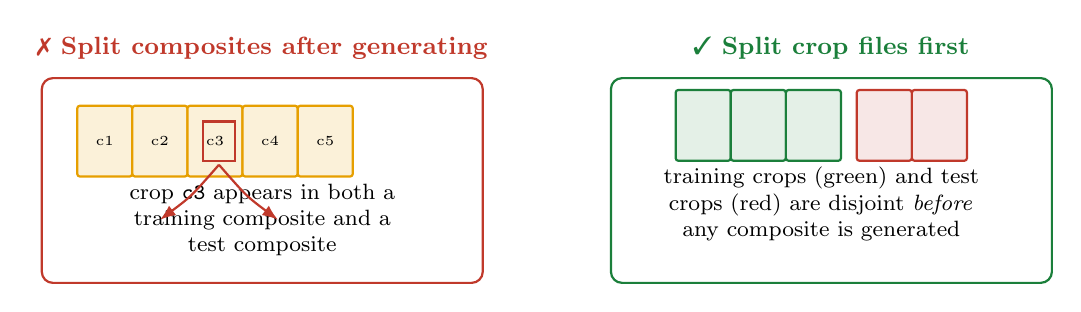
\begin{tikzpicture}[
  crop/.style={draw, thick, rounded corners=1pt, minimum width=0.7cm, minimum height=0.9cm, font=\tiny},
  panel/.style={draw, thick, rounded corners, minimum width=5.6cm, minimum height=2.6cm, align=center},
  paneltitle/.style={font=\bfseries\small}
]

% Wrong approach
\node[panel, draw=diffdel] (wrong) at (0,0) {};
\node[paneltitle, text=diffdel, above=1mm of wrong] {\ding{55}\ Split composites after generating};
\foreach \i/\x in {1/-2,2/-1.3,3/-0.6,4/0.1,5/0.8} {
  \node[crop, draw=oiOrange, fill=oiOrange!15] at (\x,0.5) {c\i};
}
\node[font=\footnotesize, align=center] at (0,-0.5) {crop \texttt{c3} appears in both a\\training composite and a\\test composite};
\draw[diffdel, thick] (-0.75,0.75) rectangle (-0.35,0.25);
\draw[diffdel, thick, -{Latex[length=2mm]}] (-0.55,0.2) .. controls (-0.9,-0.2) .. (-1.3,-0.5);
\draw[diffdel, thick, -{Latex[length=2mm]}] (-0.55,0.2) .. controls (-0.2,-0.2) .. (0.2,-0.5);

% Right approach
\node[panel, draw=diffadd, right=1.6cm of wrong] (right) {};
\node[paneltitle, text=diffadd, above=1mm of right] {\ding{51}\ Split crop files first};
\foreach \i/\x in {1/5.6,2/6.3,3/7.0} {
  \node[crop, draw=diffadd, fill=diffadd!12] at (\x,0.7) {};
}
\foreach \i/\x in {4/7.9,5/8.6} {
  \node[crop, draw=diffdel, fill=diffdel!12] at (\x,0.7) {};
}
\node[font=\footnotesize, align=center] at (7.1,-0.3) {training crops (green) and test\\crops (red) are disjoint \emph{before}\\any composite is generated};

\end{tikzpicture}
\caption{Preventing data leakage in the synthetic detector training set.
Splitting composite images after they are generated (left) allows the same
underlying crop to appear in both a training and a test composite.
Splitting the pool of crop files first, and generating each split's
composites only from its own crops (right), guarantees no crop is ever
shared between splits.}
\label{fig:data-leakage}
\end{figure}

The fix implemented in this project splits the crop \emph{files} into
training, validation, and test pools (in an 80/10/10 proportion, using a
fixed random shuffle so the split is reproducible) before any composite
image is generated at all. Composite images for the test set are then built
exclusively from the test pool's crop files, and likewise for training and
validation; no single crop file's pixels can ever appear in more than one
split's composites, regardless of how many composite images are generated
from each pool.

\subsection{Fine-tuning from a pretrained checkpoint}
\label{sec:detector-finetuning}

Training an object detector completely from a random starting point
typically needs a very large amount of training data to reach useful
accuracy, far more than the roughly 4{,}000 synthetic composites described
above could realistically provide on their own. This project instead uses
\textbf{fine-tuning}: starting from a checkpoint (a saved set of weights)
that has already been trained by someone else on a different, larger
dataset, and continuing training from there on this project's own data for
a smaller number of additional passes. Section~\ref{sec:transfer-learning}
explains the closely related idea of transfer learning in more depth, in
the context of the sign classifier; the same underlying principle applies
here.

The specific checkpoint used is a YOLOv8 (``You Only Look Once'', a common
family of real-time object detection architectures) segmentation model
published under the MIT license by a separate, unaffiliated open-source
project, already trained on real archaeological photographs of temple wall
inscriptions, obelisk carvings, papyrus documents, and stelae, achieving a
reported 70.9\% mean average precision at an overlap threshold of 0.5 (a
standard object-detection accuracy metric, abbreviated mAP@0.5, that need
not be defined further here since this project does not itself claim that
number, only starts from the checkpoint that earned it) on its own,
separate evaluation photographs. Choosing this starting point over training
from scratch is a deliberate bet: a model that has already learned what
real, weathered stone carvings generally look like should adapt faster and
generalize better to real photographs after a short additional training run
than a model that has only ever seen this project's flat synthetic
composites. Figure~\ref{fig:finetuning} shows this process end to end.

\begin{figure}[t]
\centering
\begin{tikzpicture}[
  procstep/.style={
    draw=#1, thick, rounded corners, fill=#1!8,
    minimum width=3.1cm, minimum height=1.5cm,
    align=center, font=\small, inner sep=4pt
  }
]

\node[procstep=oiOrange] (pre) {\Large\faDatabase\\[2pt] Pretrained on\\real archaeological\\photographs};
\node[procstep=oiBlue, right=1.1cm of pre] (train) {\Large\faCogs\\[2pt] Continue training\\on synthetic\\composites};
\node[procstep=oiGreen!45!black, right=1.1cm of train] (out) {\Large\faBullseye\\[2pt] Fine-tuned\\glyph detector};

\draw[arrc=oiOrange, -{Latex[length=3mm]}, ultra thick] (pre) -- (train);
\draw[arrc=oiBlue, -{Latex[length=3mm]}, ultra thick] (train) -- (out);

\node[font=\footnotesize, align=center, below=3mm of pre] {\texttt{best.pt}, MIT license\\70.9\% mAP@0.5};
\node[font=\footnotesize, align=center, below=3mm of train] {4{,}000 images,\\Section~\ref{sec:composite-synthesis}};

\end{tikzpicture}
\caption{Fine-tuning the glyph detector. Training starts from a checkpoint
already exposed to real archaeological photographs (orange), rather than
from randomly initialized weights, then continues training on this
project's synthetic composite images (blue) to specialize the model for
hieroglyph detection specifically.}
\label{fig:finetuning}
\end{figure}

\subsection{A real technical issue: mismatched label formats}
\label{sec:the-bug}

This section documents a genuine defect that was found and fixed during the
development of this stage, kept in the report as a concrete example of how
a machine learning pipeline can look correct at every individual step and
still fail, for a reason that only becomes visible when the whole pipeline
is actually run end to end.

Object detection models can be trained for (at least) two closely related
but distinct tasks. A \textbf{detection} model is trained to output plain
rectangular bounding boxes. A \textbf{segmentation} model (in the neural
network sense, not to be confused with this project's own use of
``segmentation'' for the whole find-the-glyphs stage) is trained to output
a more precise outline, a polygon tracing the exact pixels belonging to
each object, not just its enclosing rectangle. The pretrained checkpoint
described in Section~\ref{sec:detector-finetuning} is a segmentation model.
Training-data label files therefore need to be written in the
\textbf{segmentation label format}: each line names an object's class,
followed by the coordinates of a polygon outlining it. The code that
originally generated this project's training labels instead wrote the
simpler \textbf{detection label format}: each line naming an object's
class, followed by only a center position, width, and height, five numbers
in total rather than a polygon.

This mismatch produced no error anywhere in the label-writing code itself;
five plausible-looking numbers were written to every label file, and every
unit test that checked those numbers in isolation passed. The failure only
appeared when the training library (Ultralytics, the library implementing
YOLOv8) tried to actually load this training data for a segmentation model
and found that every label was missing the polygon information a
segmentation model's loader requires, raising an error and refusing to
proceed with training at all. Figure~\ref{fig:label-bug} shows the fix: a
box's own four corners, traced in order, are themselves a valid (if simple,
rectangular) polygon outlining that box, so no additional information needs
to be invented to satisfy the segmentation label format, only the same
box's coordinates need to be written out differently.

\begin{figure}[t]
\centering
\begin{tcolorbox}[
  colback=codebg, colframe=codeframe, boxrule=0.9pt,
  arc=2mm, left=8pt, right=8pt, top=6pt, bottom=6pt,
  fonttitle=\bfseries, title=Label line for one bounding box --- before / after,
  width=\linewidth
]
{\ttfamily\small
\noindent \textcolor{diffdel}{- 0 0.878125 0.837500 0.125000 0.125000}\\[3pt]
\textcolor{diffdel}{\ \ (detection format: class, center x, center y, width, height)}\\[8pt]
\textcolor{diffadd}{+ 0 0.816 0.775 0.941 0.775 0.941 0.900 0.816 0.900}\\[3pt]
\textcolor{diffadd}{\ \ (segmentation format: class, then the box's 4 corners as a polygon)}
}
\end{tcolorbox}
\caption{The label-format fix. The old line (red) gave the box's center and
size, the format a detection model's loader expects. The new line (green)
gives the same box's four corners in order (top-left, top-right,
bottom-right, bottom-left), the format the segmentation model's loader
actually requires. Both lines describe the exact same rectangle; only the
encoding changed.}
\label{fig:label-bug}
\end{figure}

This defect was caught by a whole-branch code review carried out after
every individual development task had already been reviewed and approved
on its own. No single task's review caught it, because the label-writing
code, the checkpoint-downloading code, and the training notebook that
combined the two were each written, tested, and reviewed as separate,
independently reasonable pieces of work; the mismatch only existed in how
two already-reviewed pieces fit together. The fix was verified not only by
unit tests on the label-writing function in isolation, but by constructing
a real Ultralytics segmentation dataset loader from generated training data
and confirming it accepted the new format without error, the same check
that had previously failed against the old format.

\subsection{Evaluation plan}
\label{sec:detector-evaluation}

At the time of writing, the detector described in this section has not yet
been trained; that training run, and the evaluation described here, are the
next step in the project, intended to run on a cloud GPU service since no
suitable GPU is available locally. Two separate checks are planned once
training completes. The first is quantitative: mean average precision,
computed on the held-out synthetic test composites described in
Section~\ref{sec:leakage}, giving a single number comparable across
different training runs. The second is qualitative: running both the
classical segmenter (Section~\ref{sec:classical-cv}) and the newly trained
detector on a small set of genuinely real photographs (a publicly available
40-image dataset, licensed for reuse, separate from both the training
composites and the pretrained checkpoint's own original training data) and
comparing how many glyphs each one finds. This second check exists
specifically because the quantitative score alone, measured only on
synthetic composites, cannot by itself confirm that the detector has
actually generalized to real photographs rather than to the particular
visual style of this project's synthetic backgrounds.

% =============================================================================
\chapter{Identifying Each Sign (Classification)}
\label{ch:classification}
% =============================================================================

\section{The task}

Once Chapter~\ref{ch:segmentation} has produced a bounding box for a glyph,
the pipeline crops out exactly that rectangle from the original photograph
and hands the crop to a separate model whose only job is to answer one
question: of the 171 Gardiner sign codes this project knows about, which one
is this? This is the image classification task defined in
Section~\ref{sec:detection-vs-classification}, and it is answered by a
convolutional neural network (Section~\ref{sec:cnn}) called
\textbf{ResNet18}.

\section{The dataset}
\label{sec:the-dataset}

The classifier is trained on 4{,}031 single-glyph images spanning 171
Gardiner sign classes, sourced from a published dataset matching the one
used in Franken and van Gemert's 2013 paper on automatic hieroglyph
recognition, itself photographed from the interior of the Pyramid of Unas.
Every image is a grayscale crop, 50 pixels wide by 75 pixels tall, showing
exactly one glyph with a small margin of background around it.

This dataset is not evenly distributed across its 171 classes. The most
common sign class has 448 images; the median class has only 5. Roughly 51 of
the 171 classes have fewer than 3 images each, too few to reliably hold any
back for measuring accuracy on that specific class, so those classes are
still included in training but their real-world accuracy is simply
unverified. Figure~\ref{fig:class-imbalance} shows the size of this gap in
scale. This kind of skew, where a handful of common classes have abundant
examples and most classes have only a few, is typical of a real archival
dataset rather than a dataset purpose-built for machine learning, and it is
addressed at training time, not by discarding the rare classes (discussed
in Section~\ref{sec:training-details}).

\begin{figure}[t]
\centering
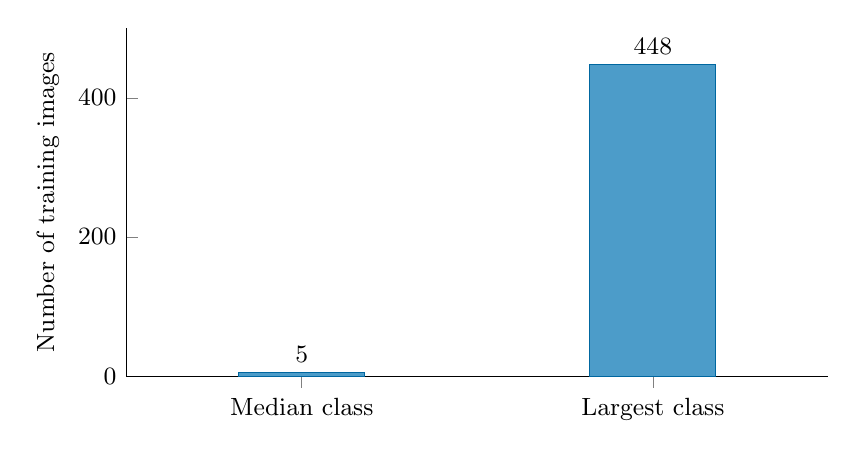
\begin{tikzpicture}
\begin{axis}[
  ybar, bar width=1.6cm,
  width=10.5cm, height=6cm,
  ylabel={Number of training images},
  symbolic x coords={Median class, Largest class},
  xtick=data,
  nodes near coords,
  ymin=0, ymax=500,
  enlarge x limits=0.5,
  axis lines*=left,
  tick label style={font=\small},
  label style={font=\small},
  nodes near coords style={font=\small}
]
\addplot[fill=oiBlue!70, draw=oiBlue!90!black] coordinates {(Median class,5) (Largest class,448)};
\end{axis}
\end{tikzpicture}
\caption{Class size imbalance in the 4{,}031-image training dataset. The
median of the 171 sign classes has only 5 training images; the single most
common class has 448, nearly two orders of magnitude more. Separately, 51 of
the 171 classes have fewer than 3 images each and therefore have no
held-out test data at all (Section~\ref{sec:the-dataset}).}
\label{fig:class-imbalance}
\end{figure}

Before training, every class's images are split independently into
training, validation, and test portions (15\% held out for validation, 15\%
for test, the remainder for training), with a guaranteed minimum of one
image in validation and one in test for any class large enough to spare
them; classes with fewer than 3 images go entirely into training, since
holding back even a single image from a 2-image class would leave nothing
meaningful to train on for that sign.

\section{Transfer learning: reusing a pretrained model}
\label{sec:transfer-learning}

Training a CNN as deep as ResNet18 (18 layers) entirely from scratch
normally needs a very large labeled dataset, typically hundreds of
thousands of images, to learn good general-purpose filters (the
edge-and-corner detectors described in Section~\ref{sec:cnn}) before it can
even start learning the specific task at hand. With only 4{,}031 training
images spread across 171 classes, training ResNet18 from scratch on this
dataset alone would not work well.

\textbf{Transfer learning} avoids this by starting from a version of
ResNet18 that has already been trained on ImageNet, a very large, widely
used dataset of 1.4 million photographs across 1{,}000 everyday object
categories (dogs, cars, chairs, and so on, none of them hieroglyphs). The
intuition: the early and middle convolutional layers of a network trained on
ImageNet have already learned to detect edges, curves, textures, and simple
shapes, which are useful visual building blocks for recognizing
\emph{any} kind of image, hieroglyphs included, even though the network has
never seen one. Only the network's final layer, the one that turns those
general-purpose features into a specific class score, is specific to the
1{,}000 ImageNet categories and needs to be replaced.

Concretely, this project's classifier is built by taking a ResNet18 already
trained on ImageNet, discarding its final layer (which produced one score
per ImageNet category), and attaching a new, untrained final layer sized
for 171 Gardiner sign classes instead. Every earlier layer keeps its
ImageNet-learned weights as a starting point; the new final layer starts
from random values and has everything left to learn. Training then proceeds
as described in Section~\ref{sec:neural-networks}, adjusting every weight in
the network, including the reused ones, though typically by much smaller
amounts than the brand-new final layer, since the reused weights are
already close to useful rather than starting from nothing.
Figure~\ref{fig:transfer-learning} shows this end to end.

\begin{figure}[t]
\centering
\begin{tikzpicture}[
  procstep/.style={
    draw=#1, thick, rounded corners, fill=#1!8,
    minimum width=3.3cm, minimum height=1.7cm,
    align=center, font=\small, inner sep=4pt
  }
]

\node[procstep=oiOrange] (pre) {\Large\faDatabase\\[2pt] ResNet18 pretrained\\on 1.4M ImageNet\\photographs\\(1{,}000 categories)};
\node[procstep=oiVermillion, right=1.2cm of pre] (swap) {\Large\faRandom\\[2pt] Replace final layer\\(1{,}000 outputs\\$\rightarrow$ 171 outputs)};
\node[procstep=oiGreen!45!black, right=1.2cm of swap] (out) {\Large\faBullseye\\[2pt] Fine-tuned on\\4{,}031 hieroglyph\\images};

\draw[arrc=oiOrange, -{Latex[length=3mm]}, ultra thick] (pre) -- (swap);
\draw[arrc=oiVermillion, -{Latex[length=3mm]}, ultra thick] (swap) -- (out);

\end{tikzpicture}
\caption{Transfer learning for the sign classifier. A ResNet18 already
trained on 1.4 million general-purpose ImageNet photographs (orange) has its
final, category-specific layer swapped out for a new one sized for 171
Gardiner sign classes (vermillion), then the whole network is fine-tuned on
this project's much smaller hieroglyph dataset (green). Every early layer's
ImageNet-learned weights are reused as a starting point, not discarded.}
\label{fig:transfer-learning}
\end{figure}

\section{Training details}
\label{sec:training-details}

Two choices made when training this classifier are worth calling out
explicitly, since both are direct responses to specific properties of
hieroglyphic signs rather than generic defaults.

\textbf{Class-weighted loss, to counter the imbalance shown in
Figure~\ref{fig:class-imbalance}.} Without correction, a model can achieve a
deceptively good-looking overall accuracy simply by becoming very good at
the handful of large classes (up to 448 images) while performing poorly on
the many small classes (as few as 1 or 2 images), since large classes
dominate the total count of training examples. Training instead weights
each class's contribution to the training signal inversely to how many
images it has, so that a mistake on a rare class counts as much as a
mistake on a common one, rather than being statistically drowned out.

\textbf{No horizontal flipping, unlike most image classifiers.} A very
common, normally harmless way to artificially expand a small image dataset
is \textbf{data augmentation}: applying small random transformations
(rotating slightly, adjusting brightness, or mirroring left-right) to each
training image so the model sees more visual variety than the raw dataset
alone provides. This project applies small random rotations (up to 5
degrees, since a real photograph is rarely taken perfectly level) and small
random brightness and contrast adjustments (simulating uneven lighting on a
stone surface), but deliberately does \emph{not} apply horizontal
mirroring, which is standard practice for most photograph classifiers. The
reason is specific to hieroglyphs: many signs are meaningfully directional
(an animal or human figure facing left carries different reading-order
information, and in some cases a genuinely different meaning, from the same
figure facing right), so mirroring a training image can silently turn it
into a misleading example of a visually similar but different sign, rather
than a harmless variation of the same sign.

\section{Results}
\label{sec:classifier-results}

The trained classifier reaches 97.3\% accuracy on its held-out test set (620
test images, drawn from the roughly 120 of 171 classes large enough to have
any test images at all, per the split described in
Section~\ref{sec:the-dataset}). Where the model does make mistakes, those
mistakes are not scattered randomly across all 171 classes; they concentrate
in small clusters of signs that are visually similar to each other, for
example the group of signs \texttt{G1}, \texttt{G17}, \texttt{G35}, and
\texttt{G4} (a cluster of bird hieroglyphs sharing a broadly similar
silhouette), and separately \texttt{M1}, \texttt{M29}, and \texttt{M17}
(plant-sign glyphs with similar overall shapes). This pattern, where
confusions cluster among genuinely similar-looking signs rather than
occurring arbitrarily, is a form of qualitative sanity check on the trained
model: a model making arbitrary, random mistakes would suggest something
had gone wrong in training, whereas a model whose few mistakes concentrate
on the pairs a human would also find visually similar is behaving the way a
reasonably well-trained classifier should.

% =============================================================================
\chapter{Putting It Together: Ordering and Looking Up Signs}
\label{ch:assembly}
% =============================================================================

Chapters~\ref{ch:segmentation} and~\ref{ch:classification} together turn a
photograph into an unordered collection of (bounding box, Gardiner code)
pairs, one per glyph found. This chapter covers the two remaining steps
that turn that unordered collection into the final, readable output: putting
the signs into a sensible reading order, and looking up each sign's
transliteration and English gloss. Figure~\ref{fig:full-pipeline} shows how
every stage covered so far in this report fits together into the complete
system.

\section{Reading order}
\label{sec:reading-order}

A photograph's glyphs are detected in no particular order (both the
classical segmenter of Section~\ref{sec:classical-cv} and the trained
detector of Section~\ref{sec:trained-detector} simply report whatever boxes
they find, in whatever order their internal processing happens to produce
them). Before the signs can be read as a list, they need to be sorted into
the order a human reader would actually read them in.

This project uses a deliberately simple rule: group the detected boxes into
horizontal rows by vertical position, then sort left to right within each
row, reading row by row from the top of the photograph to the bottom, the
same order English text is read in. Two boxes are placed in the same row if
their vertical centers are close together, specifically within a distance
proportional to the average height of the boxes already in that row (a
fraction of box height is used rather than a fixed pixel distance, since
glyphs in the same photograph can vary considerably in size, and a fixed
pixel threshold tuned for large glyphs would incorrectly merge separate rows
of much smaller ones). Figure~\ref{fig:reading-order} works through a
concrete example.

\begin{figure}[t]
\centering
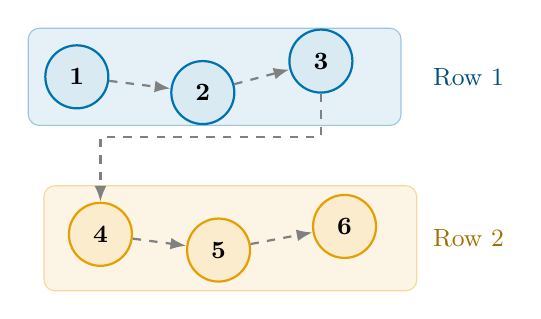
\begin{tikzpicture}[
  glyph/.style={circle, thick, minimum size=8mm, font=\bfseries\small},
  rowband/.style={rounded corners, fill=#1!10, draw=#1!40}
]

\node[rowband=oiBlue, fit={(-0.5,1.7) (4.0,2.7)}] (rowbandtop) {};
\node[rowband=oiOrange, fit={(-0.3,-0.4) (4.2,0.7)}] (rowbandbot) {};

\node[glyph, draw=oiBlue, fill=oiBlue!15] (a) at (0,2.2) {1};
\node[glyph, draw=oiBlue, fill=oiBlue!15] (b) at (1.6,2.0) {2};
\node[glyph, draw=oiBlue, fill=oiBlue!15] (c) at (3.1,2.4) {3};

\node[glyph, draw=oiOrange, fill=oiOrange!20] (d) at (0.3,0.2) {4};
\node[glyph, draw=oiOrange, fill=oiOrange!20] (e) at (1.8,0.0) {5};
\node[glyph, draw=oiOrange, fill=oiOrange!20] (f) at (3.4,0.3) {6};

\node[font=\small, text=oiBlue!70!black, anchor=west] at (4.4,2.2) {Row 1};
\node[font=\small, text=oiOrange!70!black, anchor=west] at (4.4,0.15) {Row 2};

\draw[arrc=black!50, dashed, -{Latex[length=2mm]}] (a) -- (b);
\draw[arrc=black!50, dashed, -{Latex[length=2mm]}] (b) -- (c);
\draw[arrc=black!50, dashed, -{Latex[length=2mm]}] (c.south) -- ++(0,-0.55) -| (d.north);
\draw[arrc=black!50, dashed, -{Latex[length=2mm]}] (d) -- (e);
\draw[arrc=black!50, dashed, -{Latex[length=2mm]}] (e) -- (f);

\end{tikzpicture}
\caption{Reading-order sorting. Six detected glyphs (numbered circles,
positioned where their bounding boxes were found) are first grouped into
rows by vertical proximity (blue band, orange band), then read left to
right within each row, row by row from top to bottom (dashed path). The
resulting order, 1 through 6, is the order glyphs 1-6's Gardiner codes are
concatenated into the final output.}
\label{fig:reading-order}
\end{figure}

This rule is stated plainly as an approximation, not a solved problem. Real
Egyptian hieroglyphic inscriptions do not always read top-to-bottom,
left-to-right; the true reading order can run in columns, or right-to-left,
depending on which way the signs, especially animal and human figures, are
drawn facing. Correctly following that convention would require the
classifier to also determine each sign's facing direction, which this
project's classifier does not currently do. This is documented as a known
limitation, not silently glossed over (Chapter~\ref{ch:limitations}).

\section{Looking up each sign's meaning}
\label{sec:lookup}

Once the signs are ordered, each one's Gardiner code is looked up in a
table (a spreadsheet-style file, \texttt{gardiner\_signs.csv}, hand-compiled
from Sir Alan Gardiner's 1957 published sign list and cross-checked against
this project's exact 171 trained classes) to retrieve its transliteration
and English gloss. This table is honest about its own gaps rather than
inventing plausible-looking answers to fill them: a transliteration is left
genuinely blank for signs called \textbf{determinatives}, which convey
meaning but were never assigned a sound value in the first place, and five
sign codes that either were not present in Gardiner's original 1957 list at
all, or needed a second source to resolve, are handled explicitly, four of
them left with an unresolved, empty gloss and a note rather than a guessed
meaning, and one (\texttt{O11}) resolved by cross-referencing the Unicode
17.0 standard's own hieroglyph block. If the classifier ever outputs a code
that has no entry in this table at all, which would indicate a genuine
mismatch between the classifier's class list and the lookup table rather
than an expected gap, the lookup deliberately raises a loud error instead
of silently returning an empty result, so that kind of bug cannot pass
unnoticed during development.

\section{The complete pipeline}

\begin{figure}[t]
\centering
\begin{tikzpicture}[
  procstep/.style={
    draw=#1, thick, rounded corners, fill=#1!8,
    minimum width=2.5cm, minimum height=1.25cm,
    align=center, font=\small, inner sep=3pt
  }
]

\node[grouplabel=oiBlue] (t1) at (0,2.4) {1) Detection};
\node[phase=oiBlue!70!black] (p1) at (0,1.7) {D};

\node[procstep=oiBlue] (photo) at (0,0.4) {\Large\faCamera\\[1pt] Photograph};
\node[procstep=oiBlue, right=5mm of photo] (seg) {\Large\faVectorSquare\\[1pt] Segmenter};
\node[procstep=oiBlue, right=5mm of seg] (crop) {\Large\faCrop\\[1pt] Crop Each\\Box};

\draw[arrc=oiBlue] (photo) -- (seg);
\draw[arrc=oiBlue] (seg) -- (crop);

\node[grouplabel=oiGreen!45!black] (t2) at (7.9,2.4) {2) Recognition};
\node[phase=oiGreen!35!black] (p2) at (7.9,1.7) {R};

\node[procstep=oiGreen!45!black, right=5mm of crop] (classify) {\Large\faBrain\\[1pt] Classifier\\(batched)};
\node[procstep=oiGreen!45!black, right=5mm of classify] (map) {\Large\faHashtag\\[1pt] Map to\\Gardiner Code};

\draw[arrc=oiGreen!45!black] (crop) -- (classify);
\draw[arrc=oiGreen!45!black] (classify) -- (map);

\node[procstep=oiVermillion, below=16mm of photo] (order) {\Large\faSortAmountDown\\[1pt] Sort Reading\\Order};
\node[procstep=oiVermillion, right=5mm of order] (lookup) {\Large\faBook\\[1pt] Look Up\\Gloss};
\node[procstep=oiVermillion, right=5mm of lookup] (concat) {\Large\faScroll\\[1pt] Concatenated\\Output};

\node[grouplabel=oiVermillion, below=5mm of order] (t3) {3) Assembly};
\node[phase=oiVermillion!70!black, below=2mm of t3] (p3) {A};

\draw[arrc=oiVermillion] (order) -- (lookup);
\draw[arrc=oiVermillion] (lookup) -- (concat);

\draw[arrc=oiGreen!35!black, -{Latex[length=3mm]}, ultra thick] (map.south) -- ++(0,-0.5) -| (order.north);

\end{tikzpicture}
\caption{The complete pipeline, from photograph to final output, in three
phases: detection (blue, Chapter~\ref{ch:segmentation}), recognition (green,
Chapter~\ref{ch:classification}), and assembly (vermillion,
Section~\ref{sec:reading-order} and Section~\ref{sec:lookup}). Classification
runs as one batched forward pass over every cropped box from a photograph
rather than once per box, which is substantially faster on both CPU and GPU
than looping over boxes one at a time.}
\label{fig:full-pipeline}
\end{figure}

Figure~\ref{fig:full-pipeline} shows every stage covered in this report
wired together. One detail worth stating explicitly, since it is a real
performance decision rather than an incidental implementation choice: the
classifier is run once per photograph as a single \textbf{batched} forward
pass over every cropped box found in that photograph, rather than as a
separate model call for each individual box. Modern deep learning hardware,
whether a CPU or a GPU, is substantially more efficient processing many
inputs of the same shape together in one call than processing the same
inputs one at a time in a loop of many smaller calls, so batching is a
meaningful speed advantage on a photograph containing many glyphs, at no
cost to the result.

% =============================================================================
\chapter{The Demo Application}
\label{ch:demo}
% =============================================================================

The pipeline described in Chapters~\ref{ch:segmentation}
through~\ref{ch:assembly} is exposed through a small web application built
with Streamlit, a Python framework for turning a script into an interactive
browser-based tool without writing separate frontend code. A visitor uploads
a photograph; the application runs the full pipeline from
Figure~\ref{fig:full-pipeline} on it and displays the result as an annotated
copy of the photograph (every detected glyph outlined and numbered in
reading order) alongside a card for each sign showing its Gardiner code,
transliteration, gloss, and the classifier's confidence for that particular
prediction, color-coded green, yellow, or red depending on whether that
confidence is high, medium, or low.

The application is written to reflect this report's own honesty about the
system's current limitations rather than presenting the pipeline as more
capable than it is: its sidebar states plainly, in the same terms as
Chapter~\ref{ch:limitations} of this report, that the output is not a
sentence translation, that the currently active segmenter is the classical,
non-learned one (Section~\ref{sec:classical-cv}) unless a trained detector
checkpoint (Section~\ref{sec:trained-detector}) has actually been placed on
disk, and that reading order is a simplified approximation
(Section~\ref{sec:reading-order}). The application checks, each time it
loads, whether a fine-tuned detector checkpoint file is present, and
automatically uses it in place of the classical segmenter if so, with no
code change required; this is the same \texttt{Segmenter} interface
substitution described in Section~\ref{sec:trained-detector}, made
concrete as a real runtime decision rather than a design-time one.

% =============================================================================
\chapter{Known Limitations and Future Work}
\label{ch:limitations}
% =============================================================================

This chapter states, without softening, what this system does not currently
do well. Every limitation listed here is stated elsewhere in this report at
the point it first becomes relevant; this chapter collects them in one
place for a reader who wants the honest summary first.

\begin{enumerate}[label=(\arabic*)]
  \item \textbf{This is not a sentence translator.} The output is a list of
    individual sign glosses in reading order, not fluent English prose.
    Producing an actual sentence translation would require modeling Middle
    Egyptian grammar, which this project does not attempt, and no large
    aligned hieroglyph-to-English sentence corpus exists to train such a
    system on even if it were attempted.
  \item \textbf{The classical segmenter (Section~\ref{sec:classical-cv})
    struggles on difficult photographs.} It performs well on clean,
    evenly-lit photographs but can fail on heavily weathered surfaces,
    uneven lighting, or cluttered scenes, for the reasons explained in
    Section~\ref{sec:classical-cv}. The trained detector described in
    Section~\ref{sec:trained-detector} is intended to address this, but at
    the time of writing has not yet completed training, so its real-world
    performance is not yet measured.
  \item \textbf{Reading order is an approximation.} The row-then-left-to-right
    rule described in Section~\ref{sec:reading-order} does not account for
    sign-facing direction, which genuinely determines reading order in real
    hieroglyphic inscriptions.
  \item \textbf{Roughly 51 of 171 sign classes have no verified test
    accuracy.} These classes have too few images (fewer than 3) to hold any
    back for testing (Section~\ref{sec:the-dataset}); the classifier is
    still trained on them, but how accurately it recognizes those specific
    signs in practice is unknown.
  \item \textbf{The trained detector's real-world accuracy is not yet
    known.} As of this report, the fine-tuning run described in
    Section~\ref{sec:detector-finetuning} has not yet been carried out; both
    the quantitative and qualitative evaluations described in
    Section~\ref{sec:detector-evaluation} are still pending.
\end{enumerate}

Two directions for future work follow directly from these limitations. The
most immediate is completing and evaluating the trained detector's training
run, and, if its real-photograph performance genuinely improves on the
classical segmenter's, making it the default rather than an opt-in
alternative. The second, larger direction, noted here as an open problem
rather than a committed plan, is sign-facing detection: teaching the
classifier or a separate small model to additionally report which direction
a sign faces, which would allow the reading-order stage
(Section~\ref{sec:reading-order}) to follow the actual Egyptological
convention rather than the current simplified row-major approximation.

% =============================================================================
\chapter{Summary}
% =============================================================================

This report has walked through a complete photograph-to-gloss pipeline for
Egyptian hieroglyphs, defining every machine learning concept involved from
first principles along the way. The system finds glyphs in a photograph
using either a fixed, non-learned image-processing procedure or a fine-tuned
neural object detector; identifies each found glyph using a convolutional
neural network built by adapting a model pretrained on a large, unrelated
image dataset rather than trained from nothing; and assembles the
per-glyph results into an ordered, looked-up output using explicit,
clearly-stated rules rather than another learned model. Two specific
engineering issues were documented in detail as worked examples rather than
smoothed over: the risk of data leakage in a synthetically generated
training set, and a real label-format mismatch that silently produced
plausible-looking but unusable training data until the full pipeline was
actually run end to end. The system's classifier is measured and performing
well (97.3\% test accuracy); its newer trained detector is built and ready
to train, but not yet evaluated; and its remaining known weaknesses,
sentence-level translation, reading-order accuracy on directional
inscriptions, and rare-class coverage, are stated plainly rather than
implied to be solved.

\end{document}


